\documentclass{beamer}
\usepackage[utf8]{inputenc}
\usetheme{Boadilla}
\usepackage{media9}
\usepackage{graphicx}
\usepackage{bibentry}
\usepackage{physics}
\usepackage{amsmath}
\usepackage{amsfonts}
\usepackage{bbold}
\usepackage{mathtools}
\usepackage{dsfont}
\usepackage{amsthm}
\usepackage{bbm}
\usepackage{amssymb}
\usepackage{empheq}
\usepackage{tensor}
\usepackage{hyperref}
\usepackage{xcolor}
\newcommand{\mystar}{{\fontfamily{lmr}\selectfont$\star$}}

%Information to be included in the title page:
\title{Hele-Shaw Flow \& Saffman-Taylor Instability}
\author[Brady \& Bui] % (optional)
{Conor Brady \& Huan Bui}
\institute[Colby College] % (optional)
{
	PH333: Experimental Soft-Matter Physics
	\and
	Professor Jonathan McCoy
}
\date{September, 2020}
\begin{document}
\frame{\titlepage}

%%%%%%%%%%%%%%%% SLIDES START HERE %%%%%%%%%%%%%%%%


% frame
\begin{frame}
\frametitle{Hele-Shaw flow: The person}

\begin{figure}
    \centering
    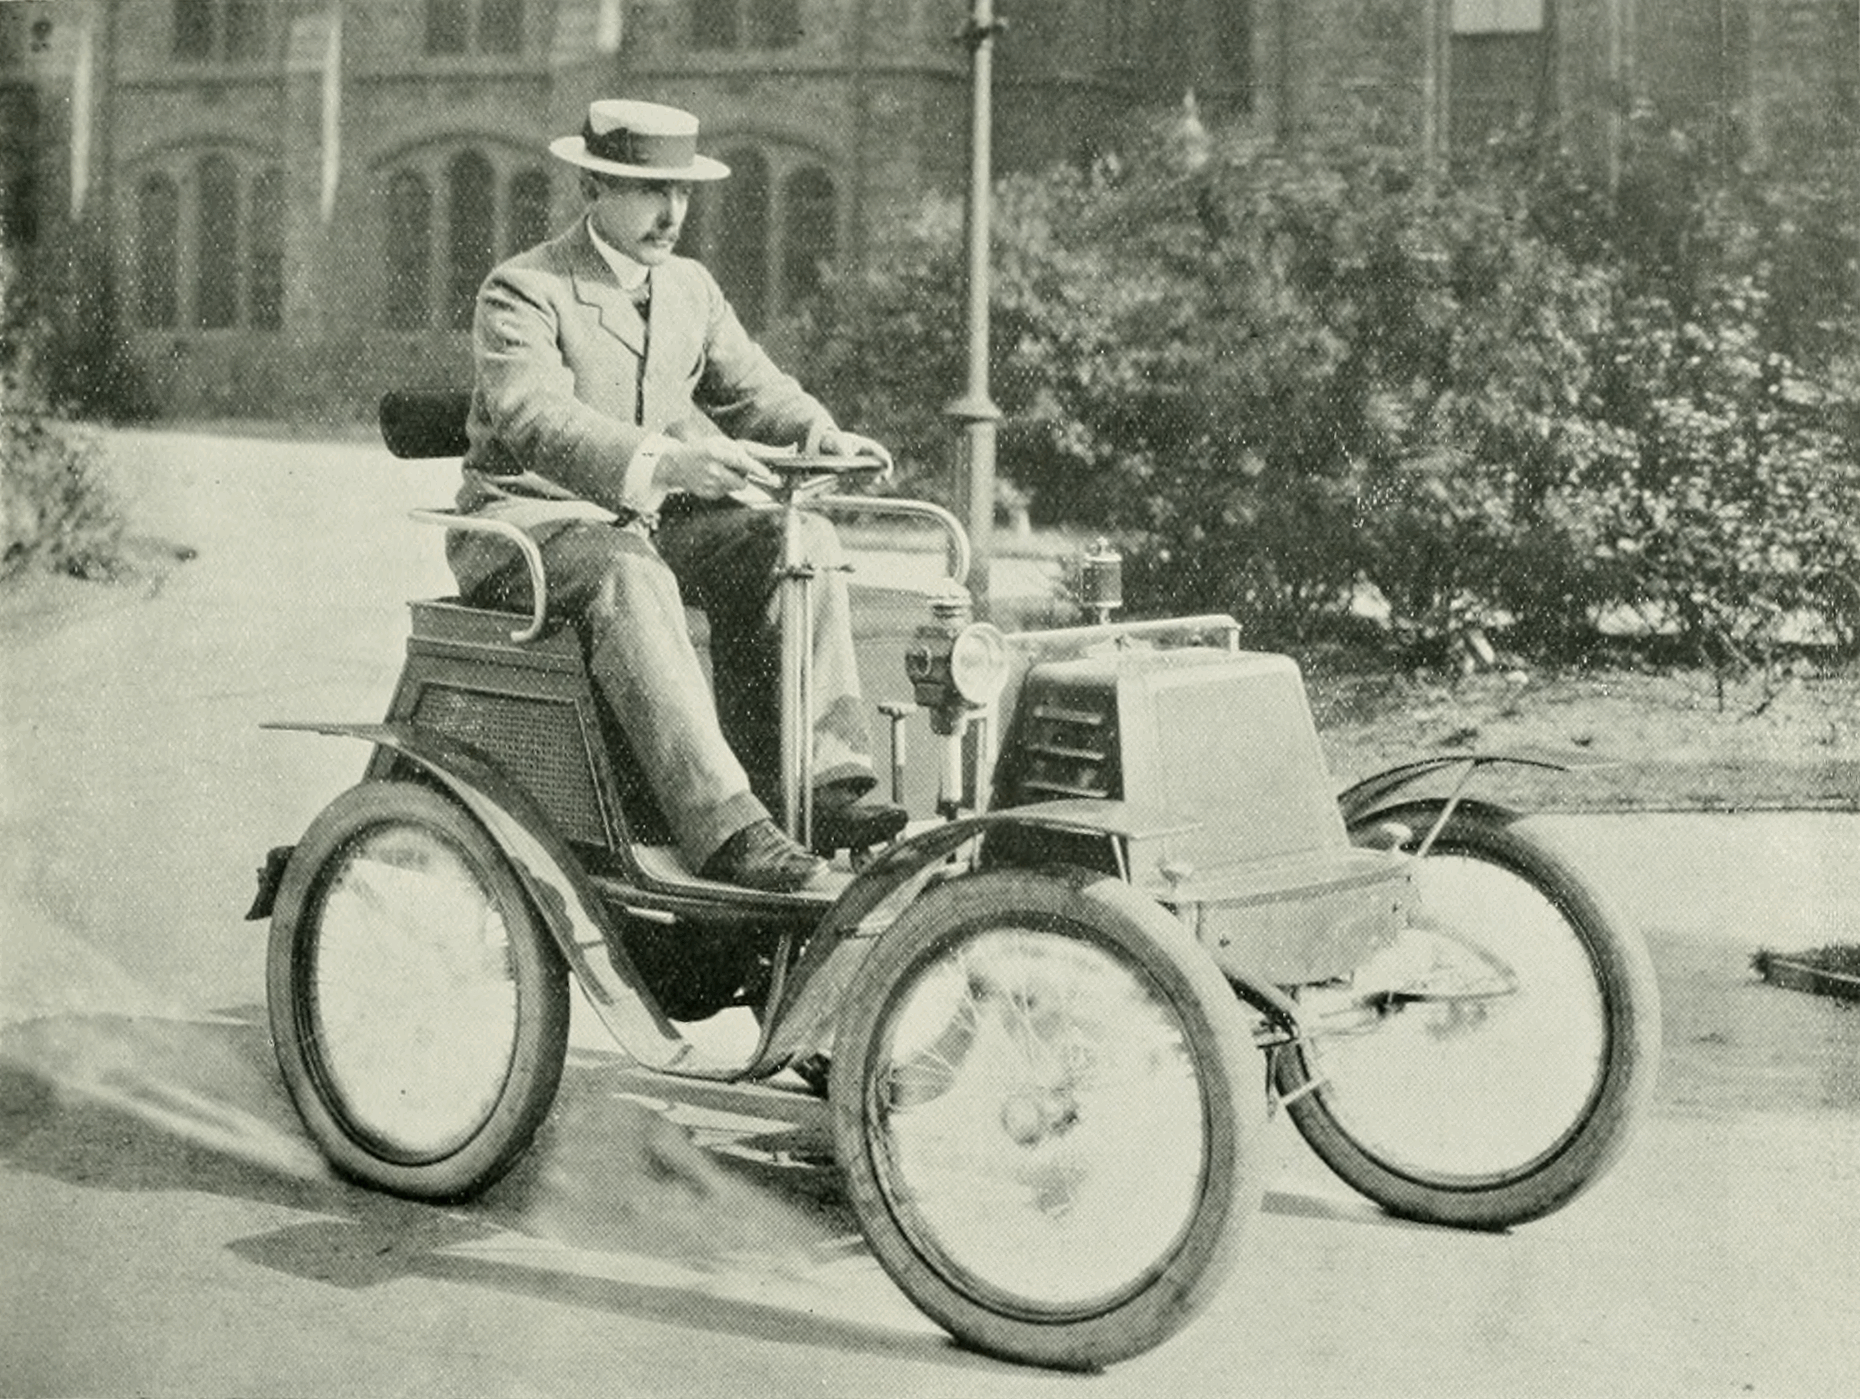
\includegraphics[scale=0.4]{HS}
    \caption{H.S. Hele-Shaw (1854–1941) \cite{HLGuy}, British engineer}
    \label{fig:HS}
\end{figure}

$\clubsuit$ Discovered the now ``Hele-Shaw cell'' while studying fluid dynamics related to laminar flow. 

\end{frame}


\begin{frame}
    \frametitle{Hele-Shaw flow: The Experiment}
    
    Experimental setup: (Source: \href{https://karnowidjaja.com/Hele-Shaw-Experiment}{\underline{\textcolor{blue}{Karno Widjaja's lab at CMU}}})
    \begin{figure}[!tbp]
    \centering
    \begin{minipage}[b]{0.4\textwidth}
    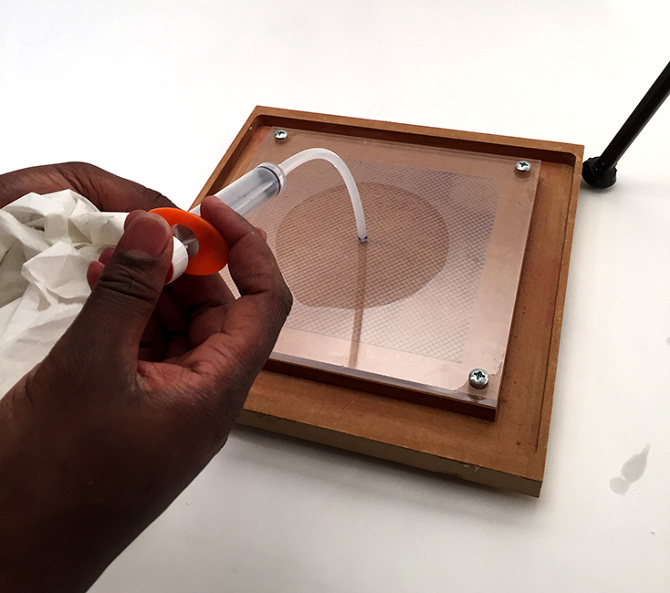
\includegraphics[scale=0.24]{cell-1.jpg}
    \caption{Before}
    \end{minipage}
    \hspace{-10pt}
    \begin{minipage}[b]{0.4\textwidth}
    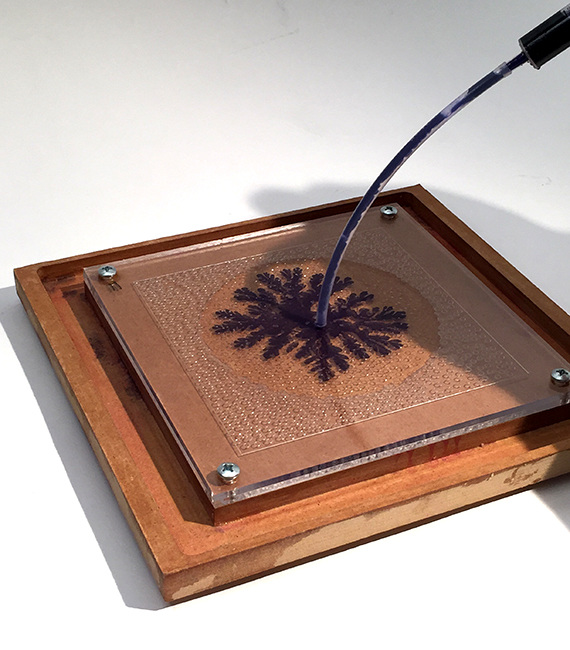
\includegraphics[scale=0.25]{cell-2.jpg}
    \caption{After}
    \end{minipage}
    \label{fig:cells}
\end{figure}
\end{frame}



\begin{frame}
\frametitle{Hele-Shaw flow: A virtual demo (\href{https://www.youtube.com/watch?v=HZ3CYY0zKGQ&ab_channel=WilliamJewellCollege}{\underline{\textcolor{black}{link}}})}

% using a YouTube video
\begin{center}
\includemedia[
  width=0.75\linewidth,height=0.5\linewidth,
  activate=pageopen,
  flashvars={
  modestbranding=1 % no YT logo in control bar
  &autohide=1 % controlbar autohide
  &showinfo=0 % no title and other info before start
  &rel=0 % no related videos after end
  }
]{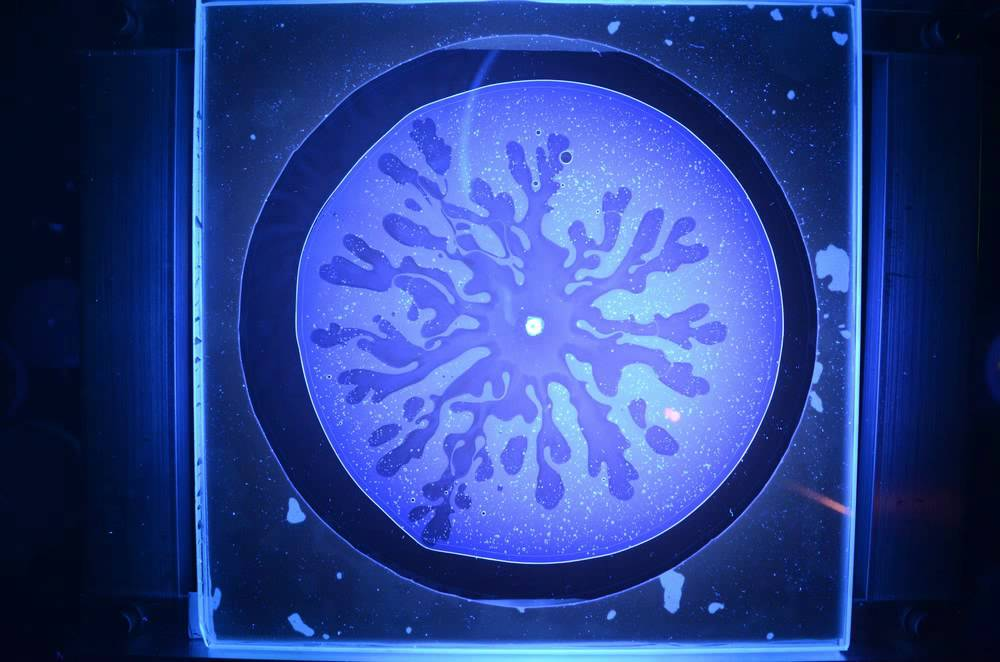
\includegraphics[width=0.75\linewidth]{ST_instability.jpg}}{https://www.youtube.com/watch?v=HZ3CYY0zKGQ&ab_channel=WilliamJewellCollege}
\end{center}
\end{frame}

%%What more should we do? Should I include more on the saffman taylor inst.

% frame
\begin{frame}
\frametitle{Hele-Shaw flow: The Physics}
Governing equation \cite{Saffman} (derived from the famous Navier-Stokes equation):
\begin{equation*}
    \boxed{\mbox{Flow: }\vec{u}(x,y) = -\frac{b^2}{12\mu} \grad \vec{p}(x,y) \quad \& \quad \mbox{Conservation law: } \grad \cdot \vec{u} = 0}
\end{equation*}
where
\begin{itemize}
    \item $\vec{u}(x,y)$: average 2D velocity of the fluid between the plates
    \item $\vec{p}(x,y)$: the pressure field
    \item $b$: the (small) gap between the two plates
\end{itemize}


\end{frame}

%% 


% frame
\begin{frame}
\frametitle{Saffman-Taylor Instability}
\begin{minipage}{.40\textwidth}
\includemedia[
  width=0.9\linewidth,height=0.7\linewidth,
  activate=pageopen,
  flashvars={
  modestbranding=1 % no YT logo in control bar
  &autohide=1 % controlbar autohide
  &showinfo=0 % no title and other info before start
  &rel=0 % no related videos after end
  }
]{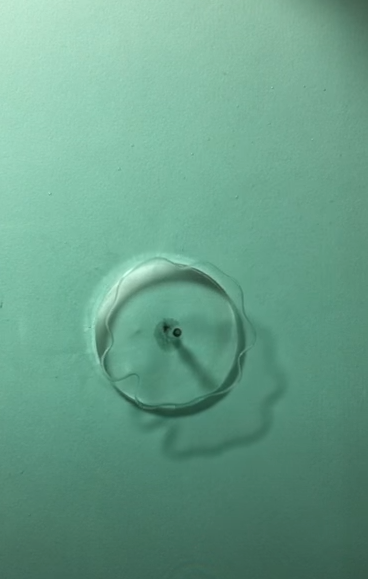
\includegraphics[width=0.7\linewidth]{Saffman_vid.PNG}}{https://www.youtube.com/watch?v=DUzdQU6uoeE}
\caption{\href{https://www.youtube.com/watch?v=DUzdQU6uoeE}{\underline{\textcolor{blue}{Link}}}}
\end{minipage}
\begin{minipage}{.55\textwidth}
At first the fluid will grow as a circle until it reaches a critical size where instabilities form on its boundary.
These instabilities come from disturbances in the liquid such as:
\begin{itemize}
    \item Pressure differences of the fluid
    \item Irregularities in the container
    \item Particulate matter in the fluid
\end{itemize}
Instabilities on the boundary form into finger-like patterns.
\end{minipage}

\end{frame}

% frame
\begin{frame}
\frametitle{Saffman-Taylor Instability}
The number of ``fingers'' is ideally proportional to the square root of the radial velocity. 
The splitting of the fingers is due to low surface tension. 
\begin{figure}
   \noindent\begin{minipage}{.45\textwidth}
   \centering
   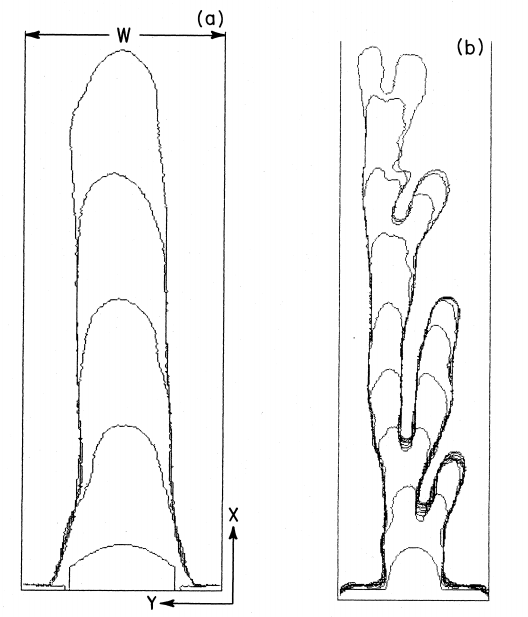
\includegraphics[scale=0.33]{Saffman_Taylor_surface_tension.PNG}
   \label{fig:dendrite}
\end{minipage}
\begin{minipage}{.45\textwidth}
\begin{align*}
   \boxed{d_0 = \frac{\pi^3}{3}\frac{b^2}{W^2}\frac{T}{\mu U}}
\end{align*}
\end{minipage}
\caption{\cite{Liang86}, \cite{Bensimon} Surface tension $d_0$ is inversely proportional to the fluid velocity $U$, thus for slower velocity (a) we see less tip-splitting and for higher velocity (b) we see defined tip-splitting emerge.}
    \hspace{10pt}
    \label{fig:ST_instability}
\end{figure}
\end{frame}



% frame
\begin{frame}
\frametitle{Not all fingers are the same!}
When the tip of a finger is disturbed, a different pattern might appear.
\begin{figure}[!tbp]
    \centering
    \begin{minipage}[b]{0.3\textwidth}
    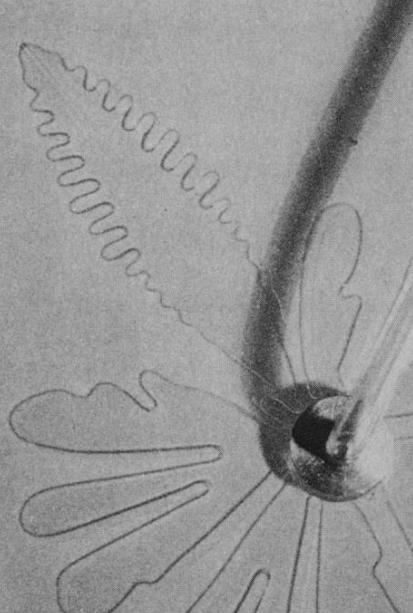
\includegraphics[scale=0.26]{finger.png}
    \end{minipage}
    \begin{minipage}[b]{0.3\textwidth}
    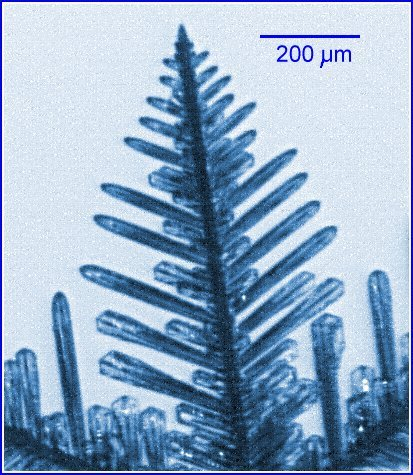
\includegraphics[scale=0.25]{dendrite.jpg}
    \end{minipage}
    \hspace{10pt}
    \begin{minipage}[b]{0.2\textwidth}
    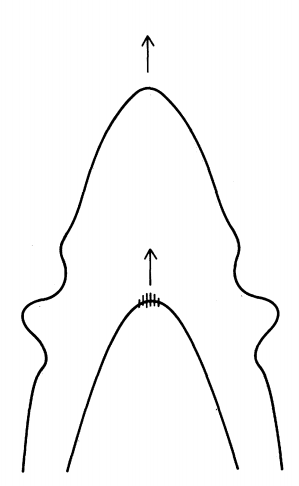
\includegraphics[scale=0.35]{dendrite_1}
    \end{minipage}
    \caption{(1) Dendrite-like finger due to a Couder's bubble \cite{Dendrite}; (2) Dendrite on a snowflake (\href{https://www.its.caltech.edu/~atomic/snowcrystals/dendrites/dendrite.htm}{\underline{\textcolor{blue}{source}}}); (3) Formation mechanism \cite{Dendrite}}
    \label{fig:cells}
\end{figure}
\end{frame}

% frame
\begin{frame}
\frametitle{Simulation: Harder than it seems}
Computer simulations of Hele-Shaw fingers is highly non-trivial, requiring complex-analytical methods \cite{Simulate}:
\begin{itemize}
    \item Approximate boundary by a polygonal
    \item Treat $\mathbb{R}^2$ as $\mathbb{C}$ and use conformal mapping
    \item Cauchy-Green coordinates (cf. CIF) to evolve the boundary
\end{itemize}
\begin{figure}[!tbp]
    \centering
    \begin{minipage}[b]{0.45\textwidth}
    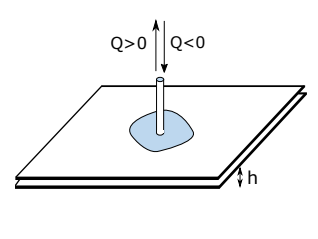
\includegraphics[scale=0.5]{sim_1.PNG}
    \end{minipage}
    \hspace{-20pt}
    \begin{minipage}[b]{0.45\textwidth}
    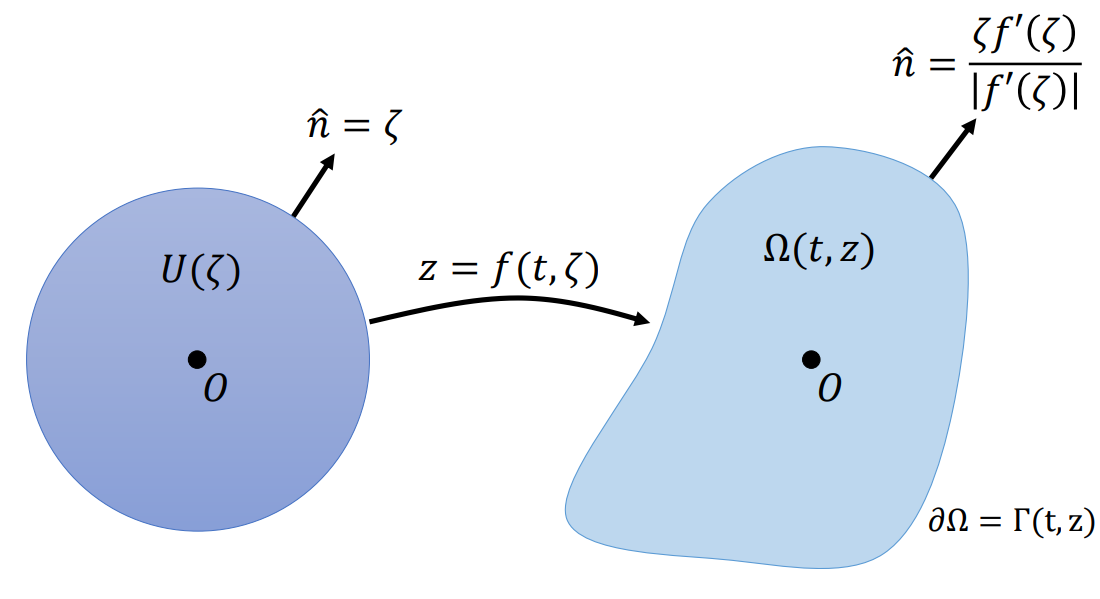
\includegraphics[scale=0.2]{sim_2.PNG}
    \end{minipage}
    \caption{\cite{Simulate} Initial setup \& Conformal mapping}
    \label{fig:simulation}
\end{figure}
\end{frame}


\begin{frame}
\frametitle{Simulation: Results}
    \begin{figure}
        \centering
        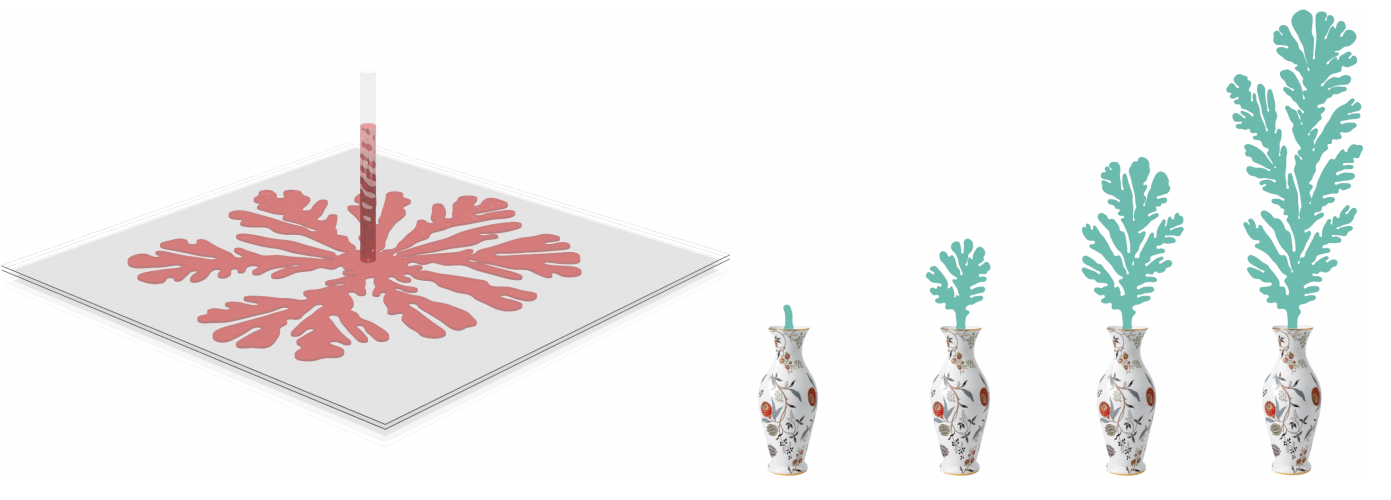
\includegraphics[scale=0.31]{sim_3}
        \caption{Computer-generated Hele-Shaw flow by \cite{Simulate}}
        \label{fig:Simulated_HS}
    \end{figure}
    
$\clubsuit$ Watch a computer-generated Hele-Shaw flow \underline{\textcolor{blue}{now}}.
\end{frame}





%%%%%%%%% SLIDES END HERE, NEXT IS REFERENCES %%%%%%%%%%%%%%

% references
\begin{frame}
\frametitle{References}
\begin{thebibliography}{99}

\bibitem{Saffman} P.G. Saffman,  \textit{Viscous fingering in Hele-Shaw cells}, J. Fluid Mech. (1986), vo1. 173, pp. 73-94

\bibitem{Bensimon} D. Bensimon, L. P. Kadanoff, S. Liang, Boris I. Shraiman, and C. Tang, \textit{Viscous flows in two dimensions}, Reviews of Modern Physics. (1988), Vol. 58, No. 4, pp. 977-999

\bibitem{HLGuy} H.L. Guy \textit{ Obituary Notices of Fellows of the Royal Society}, Dec., 1941, Vol. 3, No. 10 (Dec., 1941), pp. 790-811

\bibitem{Simulate} A. Segall, O. Vantzos, \& M. Ben-Chen,  \textit{Hele-Shaw Flow Simulation with Interactive Control using Complex Barycentric Coordinates}

\bibitem{Dendrite} J. S. Langer, \textit{Dendrites, Viscous Fingers, and the Theory of Pattern Formation}, Science, New Series, Vol. 243, No. 4895 (Mar. 3, 1989), pp. 1150-1156

\bibitem{Liang86} S. Liang, \textit{Random-walk simulations of flow in Hele Shaw cells}, Physical Review A, Vol. 33, No. 4, 1986


\end{thebibliography}


\end{frame}

%%%%%%%%%%%%%%%%%%%%%%%%%%%%%%%%%%%%%%
\end{document}

